\graphicspath{{main/chapter5/fig/}}

\chapter{Evaluations}

% \vspace*{\fill}
\minitoccustom
% \vspace*{\fill}

\section{Polar Decoders}

\subsection{Successive Cancellation - Energy and Dynamic}

\begin{table}
  \caption{Specifications of the \odr and the \juno boards.}
  \label{tab:eval_polar_energy_arm_specs}
  \begin{center}
  % {\footnotesize
  \begin{tabular}{c | c  c}
                                      & \textbf{ODROID-XU+E}      &          \textbf{\juno} \\
    \hline
    \hline
    \multirow{2}{*}{\textbf{SoC}}     &  Samsung\R Exynos\TM 5410 &               ARM64 \bl \\
                                      &           (Exynos 5 Octa) &         (dev. platform) \\
    \hline
    \multirow{1}{*}{\textbf{Arch.}}   &             32-bit, ARMv7 &           64-bit, ARMv8 \\
    \hline
    \multirow{1}{*}{\textbf{Process}} &                      28nm &  unspecified (32/28 nm) \\

    \hline
    \multirow{4}{*}{\textbf{\big}}    &       4xCortex-A15 MPCore &     2xCortex-A57 MPCore \\
                                      &        freq. [0.8-1.6GHz] &     freq. [0.45-1.1GHz] \\
                                      &        L1I 32KB, L1D 32KB &      L1I 48KB, L1D 32KB \\
                                      &                    L2 2MB &                  L2 2MB \\
    \hline
    \multirow{4}{*}{\textbf{\little}} &        4xCortex-A7 MPCore &     4xCortex-A53 MPCore \\
                                      &        freq. [250-600MHz] &      freq. [450-850MHz] \\
                                      &        L1I 32KB, L1D 32KB &      L1I 32KB, L1D 32KB \\
                                      &                  L2 512KB &                  L2 1MB \\
  \end{tabular}
  % }
  \end{center}
\end{table}

\begin{table}
  \caption{Characteristics for each cluster ($T_i$ is the information
    throughput), for dyn. decoder. $N = 4096$, rate $R = 1/2$. The RAM
    consumption is not included in $E_b$ and in $P$.}
  \label{tab:eval_polar_energy_results}
  \begin{center}
  %{\footnotesize
  \begin{tabular}{r r r r r r r}
    \textbf{Cluster} &
    \textbf{Freq. (MHz)} &
    \textbf{Impl.} &
    $\boldsymbol{T_i}$ \textbf{(Mb/s)} &
    $\boldsymbol{l}$   \textbf{($\boldsymbol{\mu}$s)} &
    $\boldsymbol{E_b}$ \textbf{(nJ)} &
    $\boldsymbol{P}$   \textbf{(W)}\\
    \hline
    \hline
    \multirow{3}{*}{A7}        & \multirow{3}{*}{ 450} & seq.  &  3.1 &  655.0 &  37.8 & 0.117 \\
                               &                       & intra & 13.0 &  158.0 &   9.5 & 0.123 \\
                               &                       & inter & 21.8 & 1506.0 &   6.0 & 0.131 \\
    \hline
    \multirow{3}{*}{A53}       & \multirow{3}{*}{ 450} & seq.  &  2.1 &  966.0 &  29.0 & 0.062 \\
                               &                       & intra & 10.1 &  203.0 &   7.0 & 0.070 \\
                               &                       & inter & 17.2 & 1902.0 &   5.1 & 0.088 \\
    \hline
    \multirow{3}{*}{A15}       & \multirow{3}{*}{1100} & seq.  &  7.5 &  274.0 & 122.0 & 0.913 \\
                               &                       & intra & 35.2 &   58.0 &  28.2 & 0.991 \\
                               &                       & inter & 62.8 &  522.0 &  17.4 & 1.093 \\
    \hline
    \multirow{3}{*}{A57}       & \multirow{3}{*}{1100} & seq.  &  9.2 &  222.0 &  78.9 & 0.730 \\
                               &                       & intra & 39.2 &   52.0 &  21.1 & 0.826 \\
                               &                       & inter & 65.1 &  503.0 &  14.2 & 0.923 \\
    \hline
    \multirow{3}{*}{i7-4850HQ} & \multirow{3}{*}{3300} & seq.  &  36.3 &   56.5 & 235.4 & 8.532 \\
                               &                       & intra & 221.8 &    9.2 &  40.5 & 9.017 \\
                               &                       & inter & 632.2 &   51.8 &  15.8 & 9.997 \\
  \end{tabular}
  %}
  \end{center}
\end{table}

Table~\ref{tab:eval_polar_energy_results} gives an overview of the decoder
behavior on different clusters and for various implementations. The code is
always single threaded and only the 8-bit fixed-point decoders are considered,
since 32-bit floating-point versions  are 4 times more energy consuming, on
average. The sequential version is mentioned for reference only, as the
throughput $T_i$ is much higher on vectorized versions. Generally the
inter-frame SIMD strategy delivers better performance at the cost of a higher
latency $l$. Table~\ref{tab:eval_polar_energy_results} also compares the energy
consumption of \little and \big clusters. The A53 consumes less energy than the
A7 and the A57 consumes less energy than the A15, respectively. This can be
explained by architectural improvements brought by the more recent ARM64
platform. Despite the fact that the ARM64 is a development board, the ARM64
outperforms the ARM32 architecture. Finally we observe that the power
consumption is higher for the inter-frame version than for the intra-frame one
because it fills the SIMD units more intensively, and the SIMD units consume
more than the scalar pipeline.

For comparison, the results for the Intel\R Core\TM i7-4850HQ, using SSE4.1
instructions (same vector length as ARM\R NEON vectors) are also included. Even
if the i7 is competitive with the ARM\R big cores in term of
\textit{energy-per-bit} ($E b$), these results show it is not well suited for
the low power SDR systems because of its high power requirements.

\begin{table}
  \caption{Comparison of 8-bit fixed-point decoders with intra-frame
    vectorization. $N = 32768$ and $R = 5/6$.}
  \label{tab:eval_polar_energy_comparison}
  \begin{center}
  %{\footnotesize
  \begin{tabular}{r r r r r r}
    \textbf{Decoder} &
    \textbf{Platform} &
    \textbf{Freq. (GHz)} &
    \textbf{SIMD} &
    $\boldsymbol{T_i}$ \textbf{(Mb/s)} &
    $\boldsymbol{l}$   \textbf{($\boldsymbol{\mu}$s)}\\
    \hline
    \hline
    \cite{Giard2014}     & i7-2600   & 3.4 & SSE4.1 &         204  &  135 \\ % \hline
    \cite{Cassagne2016b} & i7-4850HQ & 3.3 & SSE4.1 & \textbf{580} &   47 \\ % \hline
    \cite{Cassagne2016b} & A15       & 1.1 & NEON   &          70  &  391 \\ % \hline
    \cite{Cassagne2016b} & A57       & 1.1 & NEON   &          73  &  374 \\
  \end{tabular}
  %}
  \end{center}
\end{table}

Table~\ref{tab:eval_polar_energy_comparison} shows a performance comparison
(throughput, latency) with the dynamic intra-frame decoder of~\cite{Giard2014}.
On a x86 CPU, our dynamic decoder is 2.8 times faster than the state-of-the-art
decoder. Even if we used a more recent CPU, we also used the same set of
instructions (SSE4.1) and the frequencies are comparable.

\begin{figure}
  \centering
  \includegraphics[width=0.70\textwidth]{polar/sc_energy_implems_vs/sc_energy_implems_vs}
  \caption{Variation of the \emph{energy-per-bit} for different frame sizes and
    implementations: intra-/inter-frame, dyn. code on/off, on A15 @ 1.1GHz.
    Fixed rate $R = 1/2$.}
  \label{plot:eval_polar_sc_energy_implems_vs}
\end{figure}

Figure~\ref{plot:eval_polar_sc_energy_implems_vs} shows the
\emph{energy-per-bit} consumption depending on the frame size $N$ for the fixed
rate $R = 1/2$. In general, the energy consumption increases with the frame
size. For small frame sizes ($N$ from $2^{8}$ to $2^{14}$), the inter-frame SIMD
outperforms the intra-frame SIMD. This is especially true for $N = 2^8$ which
has a low ratio of SIMD computations over scalar computations in the intra-frame
version. As the frame size increases, the ratio of SIMD vs scalar computations
increases as well. At some point around $N = 2^{16}$ the intra-frame
implementation begins to outperform the inter-frame one, because the data for
the intra-frame decoder still fits in the CPU cache, whereas the data of the
inter-frame decoder does not fit the cache anymore. In our case (8-bit fixed
point numbers and 128-bit vector registers) the inter-frame decoders require
16~times more memory than the intra-frame decoders. Then, for the frame size
$N = 2^{20}$, both intra and inter-frame decoders now exceed the cache capacity
and the RAM power consumption becomes more significant due to the increased
number of cache misses causing RAM transactions. In general the code generation
is effective on the intra-frame strategy whereas it is negligible on the
inter-frame version of the code.

Considering those previous observations, it is more energy efficient to use
inter-frame strategy for small frame sizes, whereas it is better to apply
intra-frame strategy for larger frame sizes (comparable energy consumption with
much lower latency).

\begin{figure}
  \centering
  \includegraphics[width=1.00\textwidth]{polar/sc_energy_freq/sc_energy_freq}
  \caption{Variation of the \emph{energy-per-bit} ($E_b$) depending on the
    cluster frequency (dynamic code, intra-, inter-frame).
    A7 performance is on the left and A15 on the right. $N = 4096$ and $R = 1/2$.
    Dark colors and light colors stand for CPU cluster and RAM energy consumption,
    resp.}
  \label{plot:eval_polar_sc_energy_freq}
\end{figure}

Figure~\ref{plot:eval_polar_sc_energy_freq} shows the impact of the frequency on
the energy, for a given value of frame size $N=4096$ and code rate $R=1/2$. On
both A7 and A15 clusters, the supply voltage increases with the frequency from
0.946V to 1.170V. The A7 \little cluster shows that the energy consumed by the
system RAM is significant: At 250MHz it accounts for half of the energy cost.
Indeed, at low frequency, the long execution time due to the low throughput
causes a high dynamic RAM refreshing bill. It is therefore more interesting to
use frequencies higher than 250MHz. For this problem size and configuration, and
from an energy-only point of view, the best choice is to run the decoder at
350MHz. On the A15 \big cluster, the energy cost is mainly driven by the CPU
frequency, while the RAM energy bill is limited compared to the CPU.

Thus, the bottom line about energy vs frequency relationship is: On the \little
cluster it is more interesting to clock the CPU at high frequency (higher
throughput and smaller latency for a small additional energy cost); On the
\big cluster, where the RAM consumption is less significant, it is better to
clock the CPU at a low frequency.

\begin{figure}
  \centering
  \includegraphics[width=0.70\textwidth]{polar/sc_energy_rate/sc_energy_rate_N32768}
  \caption{Variation of the \emph{energy-per-bit} ($E_b$) for $N = 32768$
    depending on the rate $R = K / N$ (various impl.: intra-, inter-frame, code
    gen. on). Running on A7, A53 and A57 @ 450MHz.}
  \label{plot:eval_polar_sc_energy_rate}
\end{figure}

In Figure~\ref{plot:eval_polar_sc_energy_rate} the \emph{energy-per-bit} cost
decreases when the code rate increases. This is expected because there are many
more information bits in the frame when $R$ is high, making the decoder more
energy efficient. With high rates, the SC decoding tree can be pruned more
effectively, making the decoding process even more energy efficient.
Figure~\ref{plot:eval_polar_sc_energy_rate} also compares the ARM\R A7, A53 and
A57 clusters for the same 450MHz frequency (note: this frequency is not
available on the A15). The \little A7 is more energy efficient than the \big
A57, and the \little A53 is itself more energy efficient than the \little A7
($E_{b_{A53}} < E_{b_{A7}} < E_{b_{A57}}$).

\begin{figure}
  \centering
  \begin{tikzpicture}
  \tkzKiviatDiagram[rotate         = 90,
                    scale          = 0.70,
                    label distance = 0.5cm,
                    label space    = 5.7cm,
                    font           = \footnotesize,
                    radial         = 5,
                    gap            = 1,
                    lattice        = 4]{Larger SNR range,
                                        Lower memory footprint,
                                        Lower latency,
                                        Lower energy per bit,
                                        Higher throughput}
  \tkzKiviatLine[ultra thick,color=red,mark=none,fill=red!20,opacity=.3](4,2,1,3,3)
  \tkzKiviatLine[ultra thick,color=blue,fill=blue!20,opacity=.3](4,4,3,1,1)
  \tkzKiviatLine[dotted,ultra thick,color=blue](2,3,4,2,2)
  \tkzKiviatLine[dotted,ultra thick,color=red](2,1,2,4,4)
  \end{tikzpicture}
  \caption{\label{fig:eval_polar_sc_colgate}Ranking of the different approaches
    along 5 metrics. In red, inter-frame vectorization performance and in blue,
    intra-frame performance. Solid color is for the dynamic versions, dotted is
    for the generated versions. Each version is sorted along each of the 5 axes
    and the best version for one axe is placed further from the center.}
\end{figure}

Figure~\ref{fig:eval_polar_sc_colgate} presents a qualitative summary of the
characteristics of the different code versions, for intra-/inter-frame
vectorization, generated or dynamic code. For instance, if the size of
the memory footprint is an essential criterion, the dynamic intra-frame
code exhibits the best performance.

To sum up, the dynamic implementations provides efficient trade-off between
throughput, latency and energy depending on code length. It was demonstrated by
previous benchmarks. Both implementations provide low-energy and low-power
characteristics compared to previous works in the field on x86 processors
\cite{Sarkis2014,Giard2014,Sarkis2014a,LeGal2014,LeGal2015a,Cassagne2015c}.
Whereas the throughput on a single processor core is reduced compared to x86
implementations, ARM\R implementations must fulfil a large set of SDR
applications with limited throughputs and where the power consumption matters.
Finally, it is important to notice that multi-core implementations of the
proposed ARM\R decoders is still possible on these ARM\R targets to improve the
decoding throughputs.

\subsection{Successive Cancellation - inter/intra-SIMD Generated (aka Unrolled)}

In this section we first describe the protocol we used, after that we provide a
performance comparison between the state-of-the-art and P-EDGE. At the end we
discuss the exploring capabilities of our framework.

\begin{table}
  \begin{center}
  %{\scriptsize
  \begin{tabular}{c | c c c}
                                     & \textbf{x86-based}     & \textbf{ARMv7-based} & \textbf{prev. work arch.}\cite{Sarkis2014} \\
  \hline
  \hline
  \multirow{2}{*}{\textbf{CPU}}      & Intel\R Xeon\TM E31225 & ARM\R Cortex-A15     & Intel\R Core\TM i7-2600 \\
                                     & 3.10Ghz                & MPCore~2.32GHz       & 3.40GHz                 \\
  \hline
  \multirow{2}{*}{\textbf{Cache}}    & 32KB L1I/L1D,          & 32KB L1I/L1D,        & 32KB L1I/L1D,           \\
                                     & 256KB L2, 6MB L3       & 1024KB L2, No L3     & 256KB L2, 8MB L3        \\
  \hline
  \multirow{1}{*}{\textbf{Compiler}} & GNU g++~4.8            & GNU g++~4.8          & GNU g++~4.8             \\
  % \hline
  % Flags for 32-bit& \verb|-std=c++11 -Ofast -funroll-loops -mavx|\\
  % Flags for 8-bit & \verb|-std=c++11 -Ofast -funroll-loops -msse4.1|\\
  \end{tabular}
  %}
  \end{center}
  \caption{Performance evaluation platforms.}
  \label{tab:eval_polar_sc_gen_thr_specs}
  % \vspace{-1.5em}
\end{table}



The platforms used for performance evaluation are shown in
Table~\ref{tab:eval_polar_sc_gen_thr_specs}. Unless stated otherwise, each
measure is obtained as the best of ten runs of a 10~second simulation, taking
into account frame loading and result storing. SNR (Signal Noise Ratio) is set
to 2.5~dB for tests with 1/5 and 1/2 rates, and to 4.0 dB for the 5/6, 0.84, and
9/10 rate tests. Colors differentiate the codes rates of the Polar Code, point
shapes differentiate decoder types (Intra-SIMD vs Inter-SIMD).

\subsubsection{Comparison between P-EDGE and the State of the Art}

\begin{figure}
  \includegraphics[width=1.00\textwidth]{polar/sc_gen_thr_intra/sc_gen_thr_intra}
  \caption{Performance comparison between several code rates of 32-bit floating
    point decoding stages (running on the Intel\R Xeon\TM CPU E31225 and,
    respectively, on the Nvidia\R Jetson TK1\TM CPU A15).}
  \label{plot:eval_polar_sc_gen_thr_intra}
\end{figure}

\begin{table}
  \begin{center}
  \begin{tabular}{r  r  r  r}
    $\bm{(N, K)}$                   & \textbf{Decoder}     & \textbf{Info T/P} (Mb/s) & \textbf{Latency} ($\mu$s)\\
    \hline
    \hline
  %%this performance is included in the graphs
  % \multirow{2}{*}{(2048, 1024)}   & \cite{Sarkis2014}    & 147                      & 7               \\
  %                                 & \cite{Cassagne2015c} & 195                      & 5               \\
  % \hline
  %%this performance is included in the graphs
  % \multirow{2}{*}{(2048, 1707)}   & \cite{Sarkis2014}    & 335                      & 5               \\
  %                                 & \cite{Cassagne2015c} & 402                      & 4               \\
  % \hline
    \multirow{2}{*}{(16384, 14746)} & \cite{Sarkis2014}    & 292                      & 50              \\
                                    & \cite{Cassagne2015c} & 341                      & 43              \\
    \hline
    \multirow{2}{*}{(32768, 27568)} & \cite{Sarkis2014}    & 220                      & 125             \\
                                    & \cite{Cassagne2015c} & 241                      & 114             \\
    \hline
    \multirow{2}{*}{(32768, 29492)} & \cite{Sarkis2014}    & 261                      & 113             \\
                                    & \cite{Cassagne2015c} & 293                      & 101             \\
  \end{tabular}
  \end{center}
  \caption{Comparing P-EDGE with a state-of-art software polar decoder, for
    codes of rate 0.84 and rate 0.9, using Intra-SIMD. The two cross marks show
    state-of-the art performance results reported in~\cite{Sarkis2014}, for
    comparison.}
  \label{tab:eval_polar_sc_gen_thr_comparison}
\end{table}

\begin{figure}
  \includegraphics[width=1.00\textwidth]{polar/sc_gen_thr_inter/sc_gen_thr_inter}
  \caption{Performance comparison between several code rates of 8-bit fixed
    point decoding stages (running on the Intel\R Xeon\TM CPU E31225 and,
    respectively, on the Nvidia\R Jetson TK1\TM CPU A15). Circles show P-EDGE
    results. Triangles show our former ``handwritten'' implementation
    results~\cite{LeGal2015a}.}
  \label{plot:eval_polar_sc_gen_thr_inter}
\end{figure}

Fig.~\ref{plot:eval_polar_sc_gen_thr_intra} shows P-EDGE intra-frame throughput
on different architectures. Our generic framework performance outperforms
previous work decoder results (between 10\% and 25\% higher). This is confirmed
in Tab.~\ref{tab:eval_polar_sc_gen_thr_comparison} which compares P-EDGE with
the state-of-the-art result samples for some specific rates reported
in~\cite{Sarkis2014}. The throughput of the inter-frame implementation is shown
in Figure~\ref{plot:eval_polar_sc_gen_thr_inter} for different architectures.
Again, the results confirm that our generic approach overtakes handwritten code
(also between 10\% and 25\% higher on x86).

\begin{figure}
  \centering
  \subfloat[][Without compression.]{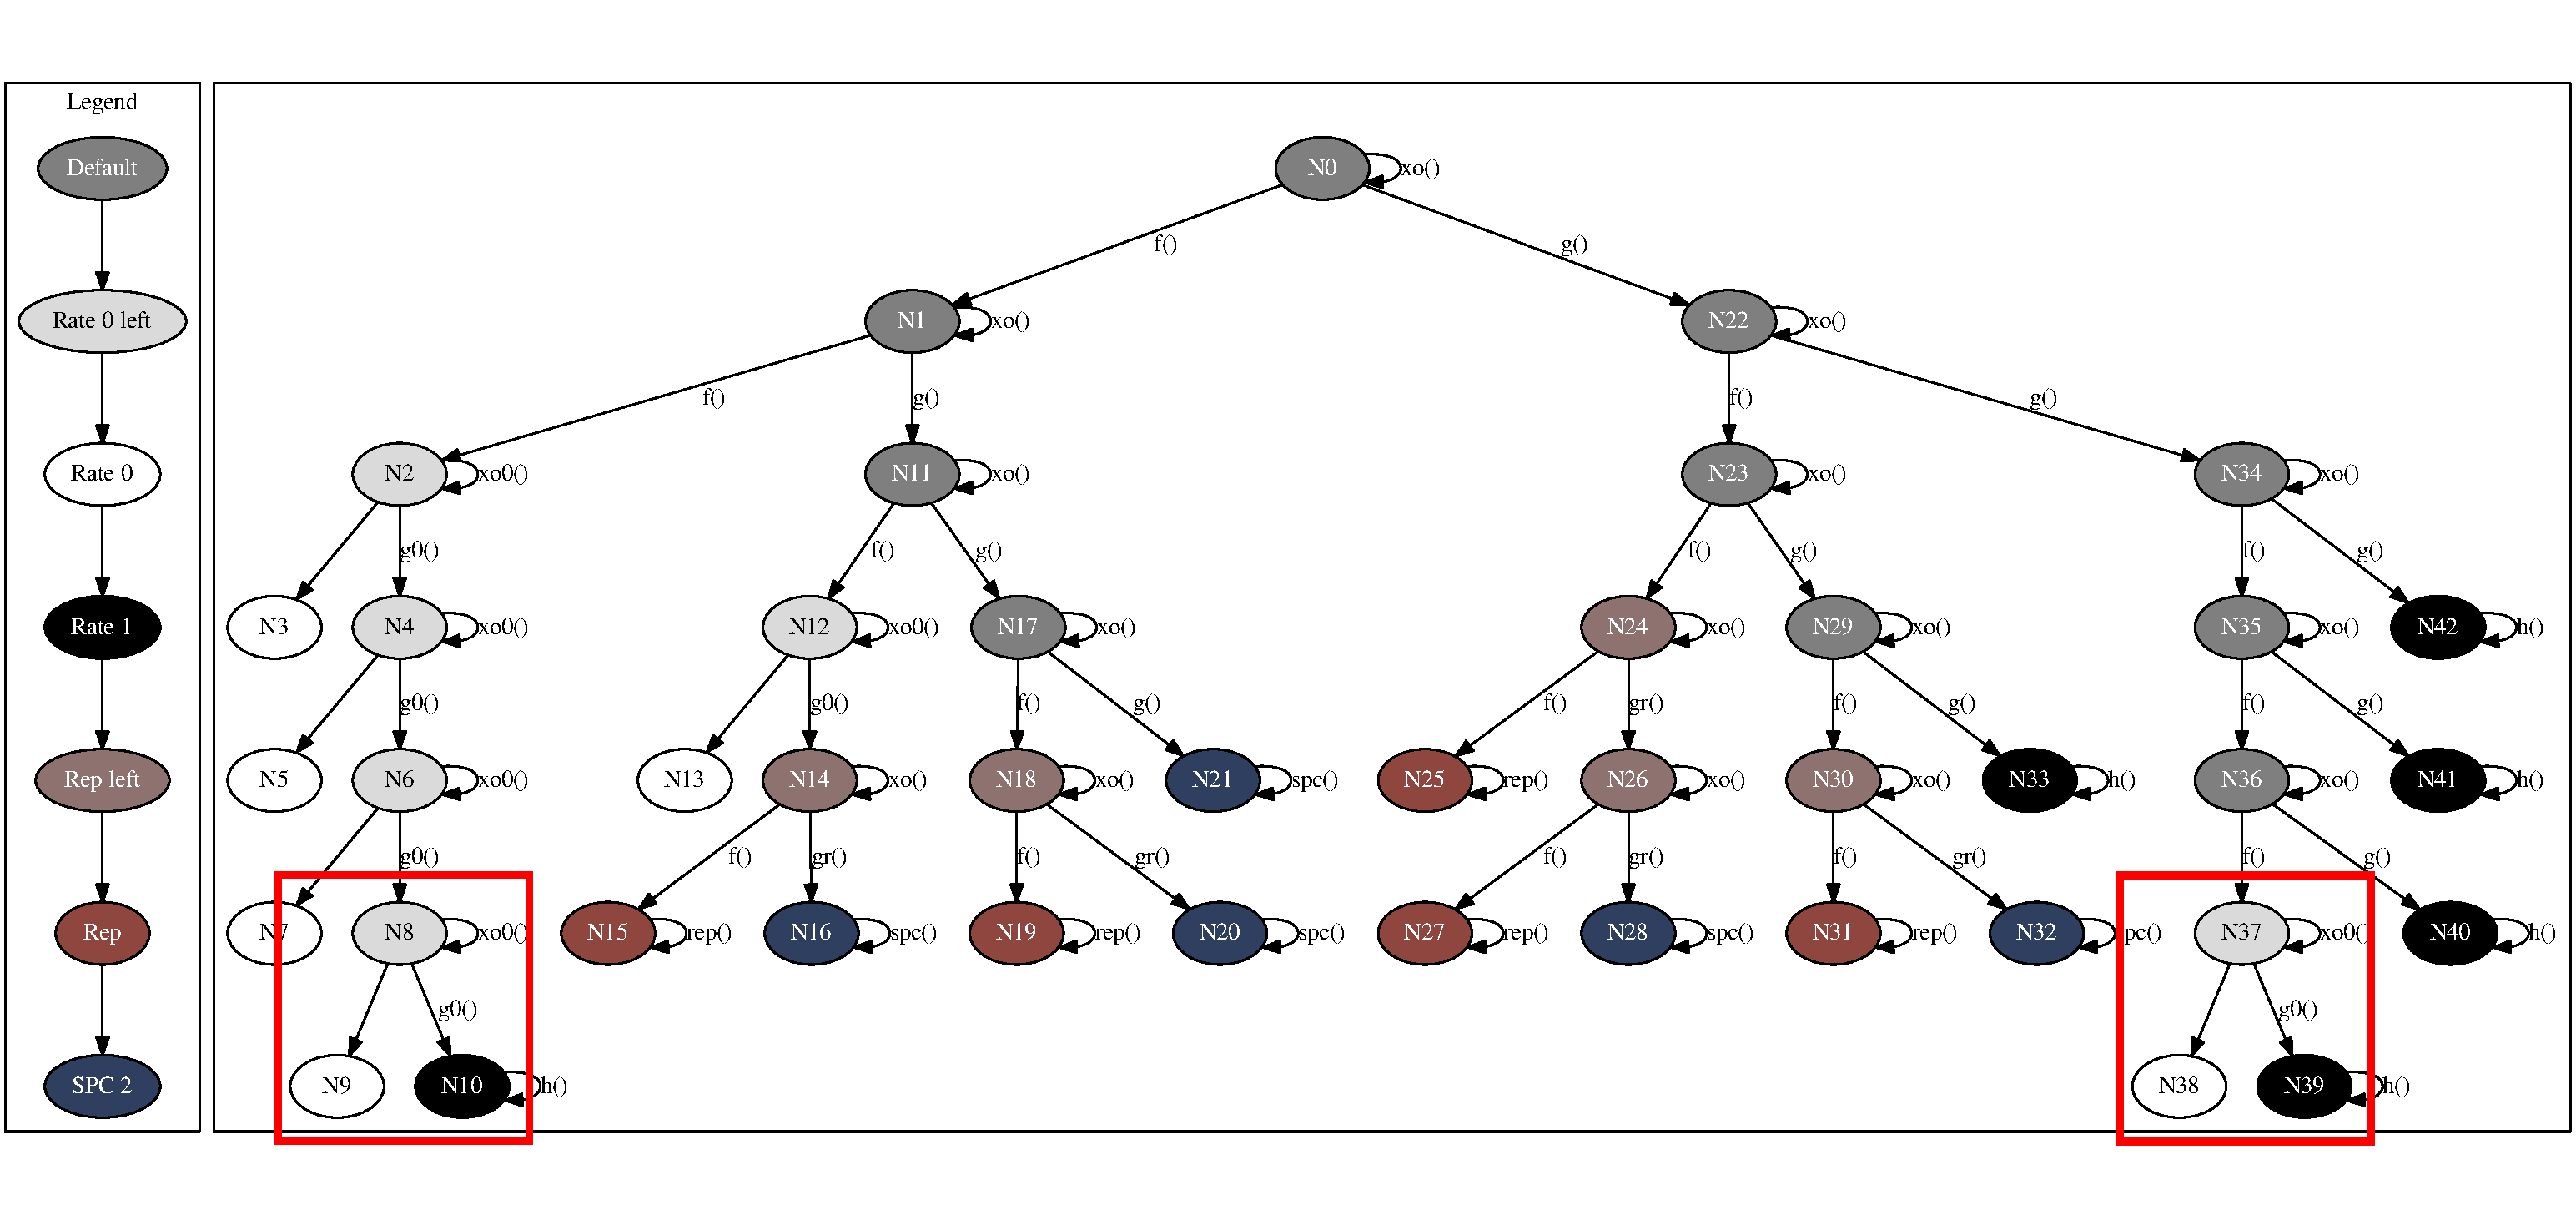
\includegraphics[height=6.0cm]{polar/sc_gen_compression/sc_gen_no_compression}\label{fig:eval_polar_sc_gen_compression_wo}}
  % \qquad
  \\
  \subfloat[][With compression.]{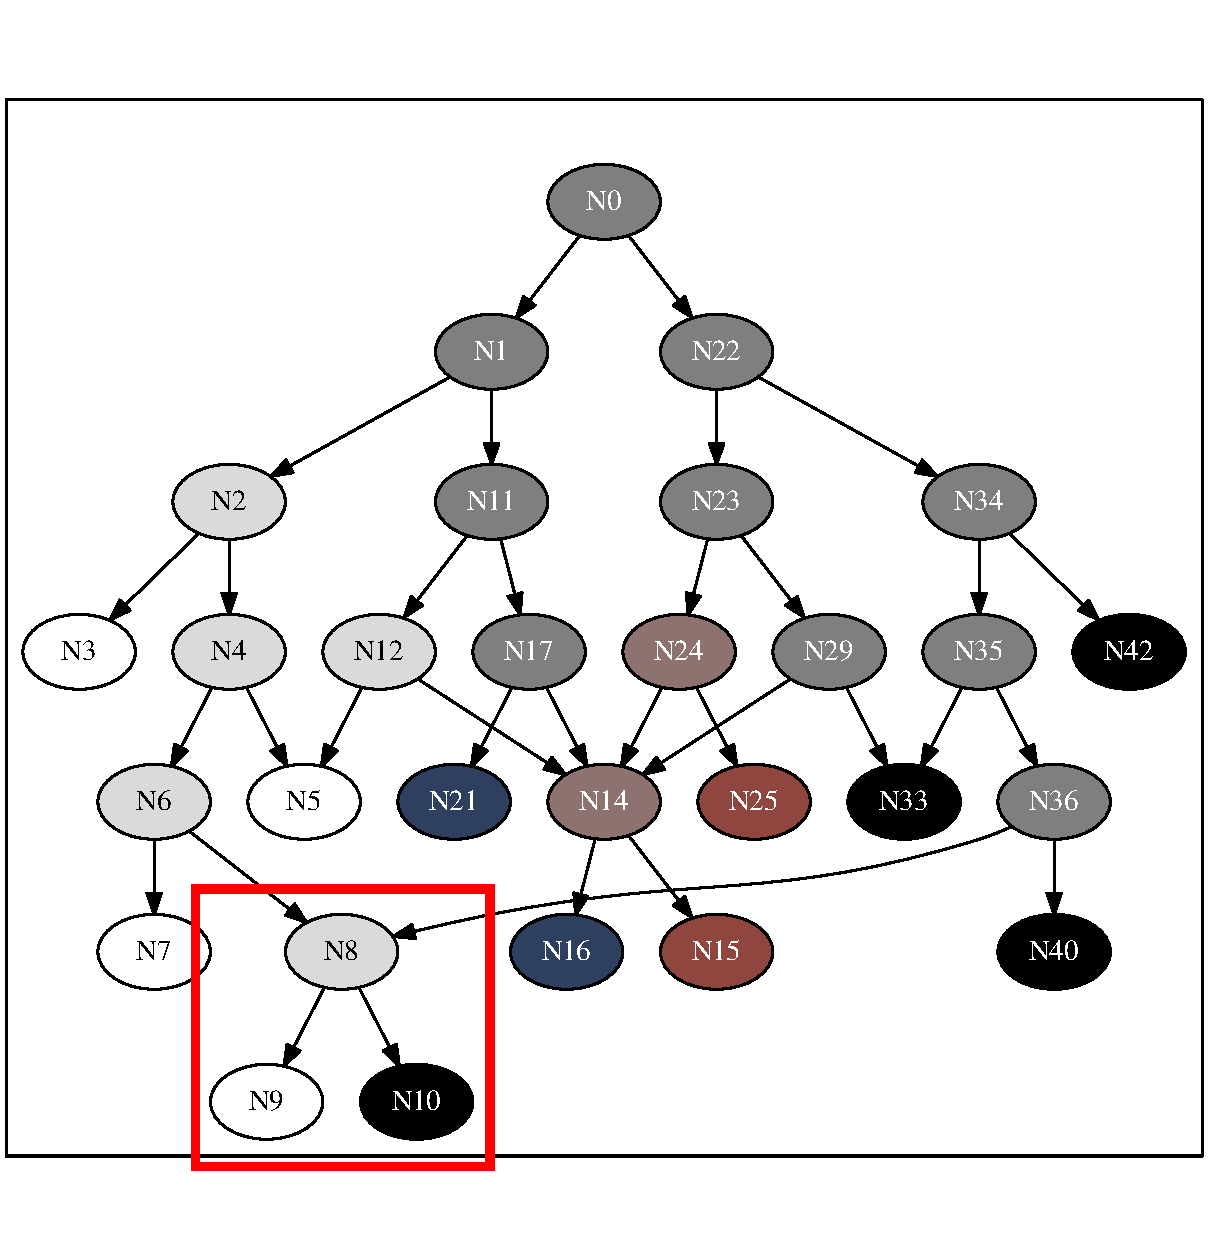
\includegraphics[height=6.0cm]{polar/sc_gen_compression/sc_gen_compression}\label{fig:eval_polar_sc_gen_compression_w}}
  \caption{Full decoding tree representation ($N = 128, K = 64$) without and
    with the compression sub-tree folding algorithm.}
  \label{fig:eval_polar_sc_gen_compression}
\end{figure}

For all the test series, the bandwidth first increases with codeword size, as
the tree pruning becomes increasingly more effective with larger trees. The
effect is stronger for Intra-SIMD where pruning also results in removing
inefficient scalar nodes. However, beyond a codeword size point which depends on
the architecture and on the selected SIMD version, performance decreases again
due to L1 cache misses, not only L1D but L1I as well. Indeed, decoders are
generated as straight-line code (no recursive calls), with all node computations
put in sequence. This improves performance for small to medium codeword size, up
to the point where the compiled binary exceeds the L1I cache size. We mitigated
this issue by reducing decoder binary sizes using two compression techniques: 1)
in the generated code, we moved the buffer offsets from template arguments to
function arguments, which enabled the compiler to factorize more function calls
than before (improvement by a factor of 10), 2) we implemented a sub-tree
folding algorithm in the generator (see
Fig.~\ref{fig:eval_polar_sc_gen_compression}), to detect multiple occurrences of
a same sub-tree and to put the corresponding code into a dedicated function
(improvement by a factor of 5 for $N=2^{16}$, the compression ratio increases
with the size of the tree).

\begin{table}
  \begin{center}
  \begin{tabular}{r r r r r r r}
    \textbf{Decoder}         & $\bm{N = 2^6}$ & $\bm{N = 2^8}$ & $\bm{N = 2^{10}}$ & $\bm{N = 2^{12}}$ & $\bm{N = 2^{14}}$ & $\bm{N = 2^{16}}$           \\
    \hline
    \hline
    inter 32-bit, $R = 1/2$  & 1 (7)          & 2 (24)         & 7 (\textbf{77})   & 9 (\textbf{254})  & 19 (\textbf{736}) & \textbf{40} (\textbf{2528}) \\
    % \hline
    inter 32-bit, $R = 5/6$  & 1 (4)          & 2 (19)         & 4 (\textbf{53})   & 7 (\textbf{167})  & 16 (\textbf{591}) & 32          (\textbf{1758}) \\
    % \hline
    intra 32-bit, $R = 1/2$  & 1 (4)          & 3 (16)         & 9 (\textbf{56})   & 8 (\textbf{182})  & 19 (\textbf{563}) & \textbf{38} (\textbf{1947}) \\
    % \hline
    intra 32-bit, $R = 5/6$  & 1 (3)          & 3 (13)         & 6 (\textbf{38})   & 7 (\textbf{126})  & 20 (\textbf{392}) & 27          (\textbf{1365}) \\
    % \hline
    inter ~8-bit, $R = 1/2$  & 1 (5)          & 2 (22)         & 7 (\textbf{72})   & 8 (\textbf{252})  & 17 (\textbf{665}) & \textbf{36} (\textbf{2220}) \\
    % \hline
    inter ~8-bit, $R = 5/6$  & 1 (4)          & 2 (18)         & 4 (\textbf{51})   & 6 (\textbf{191})  & 14 (\textbf{461}) & 26          (\textbf{1555}) \\
  \end{tabular}
  \end{center}
  \caption{Code size (in KB) of the generated decoders depending on the number
    of bits $N$ per frame (code respectively compiled with AVX instructions for
    the 32-bit decoders and with SSE4.1 instructions for the 8-bit decoders).
    For comparison, code size without compression are shown in parentheses.}
  \label{tab:eval_polar_sc_gen_l1i_size}
\end{table}

\begin{figure}
  \includegraphics[width=1.00\textwidth]{polar/sc_gen_l1i_size/sc_gen_l1i_size}
  \caption{P-EDGE generated decoder binary sizes depending on the frame size
    (R=1/2).}
  \label{plot:eval_polar_sc_gen_l1i_size}
\end{figure}

Table~\ref{tab:eval_polar_sc_gen_l1i_size} and
Fig.~\ref{plot:eval_polar_sc_gen_l1i_size} show the binary code size of the
decoders depending on $N$. The results which exceed the 32KB of the L1I cache
are highlighted in bold font. Sub-tree folding was enabled starting from
$N=2^{12}$ because there is an overhead (at run-time) when using this technique.
P-EDGE decoder code sizes without compression are shown in parentheses: we can
observe a huge improvement, until $N=2^{14}$ the code size never exceeds the L1I
cache anymore.

\subsection{Successive Cancellation List - Experiments and Measurements}

Throughput and latency measurements are detailed in this section. The proposed
decoder implementation is compared with the previous software decoders. Despite
the additional levels of genericity and flexibility, the proposed implementation
is very competitive with its counterparts. Note that all the results presented
in the following can be reproduced with the \AFFECT tool.

During our investigations, all the throughput and latency measurements have been
obtained on a single core of an Intel\R Core\TM i5-6600K CPU (Skylake
architecture with AVX2 SIMD) with a base clock frequency of 3.6 GHz and a
maximum turbo frequency of 3.9 GHz. The description has been compiled on Linux
with the C++ GNU compiler (version 5.4.0) and with the following options:
\verb|-Ofast -march=native -funroll-loops|.

\subsubsection{Fully Adaptive SCL}

Being able to easily change the list size of the SCL decoders enables the use of
the FA-SSCL algorithm. With an unrolled decoder as proposed
in~\cite{Sarkis2016}, the fully adaptive decoder would imply to generate a fully
unrolled decoder for each value of the list depth. In our work, only one source
code gives the designer the possibility to run each variation of the SCL
decoders. FA-SSCL algorithm is the key to achieve the highest possible
throughput. As shown in Table~\ref{tab:eval_polar_scl_perfs_fixed}, with an
8-bit fixed point representation of the decoder inner values, the achieved
throughput in the case of the ($2048$,$1723$) polar code is about $425$ Mb/s on
the i5-6600K for an $E_b/N_0$ value of $4.5$ dB. It corresponds to a FER of
$5\times10^{-8}$. This throughput is almost 2 times higher than the throughput
of the PA-SSCL algorithm. The highest throughput increase from PA-SSCL to
FA-SSCL, of about $380\%$, is in the domain where the FER is between $10^{-3}$
and $10^{-5}$. It is the targeted domain for wireless communications like LTE or
5G. In these conditions, the throughput of FA-SSCL algorithm is about $227$ Mb/s
compared to $42$ Mb/s for the PA-SSCL algorithm.

In Adaptive SCL algorithms, the worst case latency is the sum of the latency of
each triggered algorithm. In the case of PA-SSCL with $L_{max}=32$, it is just
the sum of the latency of the SC algorithm, plus the latency of the SCL
algorithm with $L=32$. In the case of the FA-SSCL algorithm, it is the sum of
the decoding latency of the SC algorithm and all the decoding latencies of the
SCL algorithm for $L={2,4,8,16,32}$. This is the reason why the worst latency of
the PA-SSCL algorithm is lower while the average latency and consequently the
average throughput is better with the FA-SSCL algorithm.

\subsubsection{Comparison With State-Of-The-Art SCL Decoders}

\begin{table}
  \centering
  \caption{Throughput and latency comparison with state-of-the-art SCL decoders.
    32-bit floating-point representation. Code (2048,1723), $L = 32$, 32-bit
    CRC.}
  \label{tab:eval_polar_scl_perfs_comparison}
  %{\small\resizebox{\linewidth}{!}{
  \begin{tabular}{r r r r r r r}
    \multirow{2}{*}{\textbf{Target}} & \multirow{2}{*}{\textbf{Ref.}}        & \multirow{2}{*}{\textbf{Decoder}} & \multirow{1}{*}{\textbf{$\bm{\mathcal{L}_{worst}}$}} & \multicolumn{3}{c}{$\bm{\mathcal{T}_i}$ (Mb/s)} \\
    \cline{5-7}
                                     &                                       &                                   & ($\mu s$)                         & \textbf{3.5 dB} & \textbf{4.0 dB} & \textbf{4.5 dB} \\
    \hline
    \hline
    \multirow{3}{*}{i7-2600}         & \multirow{3}{*}{\cite{Sarkis2014b}}   & CA-SCL                            & 23000                             &  0.07           &  0.07           &   0.07          \\
                                     &                                       & CA-SSCL                           &  3300                             &  0.52           &  0.52           &   0.52          \\
                                     &                                       & PA-SSCL                           & $\approx$ 3300                    &  0.90           &  4.90           &  54.00          \\
    \hline
    \multirow{1}{*}{i7-4790K}        & \cite{Shen2016}                       & CA-SCL                            &  1572                             &  1.10           &  1.10           &   1.10          \\
    \hline
    \multirow{3}{*}{i7-2600}         & \multirow{3}{*}{\cite{Sarkis2016}}    & CA-SCL                            &  2294                             &  0.76           &  0.76           &   0.76          \\
                                     &                                       & CA-SSCL                           &   433                             &  4.00           &  4.00           &   4.00          \\
                                     &                                       & PA-SSCL                           & $\approx$ 433                     &  8.60           & 33.00           & 196.00          \\
    \hline
%   original data
%   \multirow{4}{*}{E5-2650}         & \multirow{4}{*}{\cite{Leonardon2019}} & CA-SCL                            &  6554                             &  0.27           &   0.27          &   0.27          \\
%                                    &                                       & CA-SSCL                           &  1048                             &  1.67           &   1.67          &   1.67          \\
%                                    &                                       & PA-SSCL                           & $\approx$ 1048                    &  4.07           &  22.90          & 124.10          \\
%                                    &                                       & FA-SSCL                           & $\approx$ 2096                    & 14.30           & 109.80          & 180.00          \\
%   \hline
%   rescaled data from E5-2650
    \multirow{4}{*}{i7-2600}         & \multirow{4}{*}{\cite{Leonardon2019}} & CA-SCL                            &  4819                             &  0.37           &   0.37          &   0.37          \\
                                     &                                       & CA-SSCL                           &   770                             &  2.30           &   2.30          &   2.30          \\
                                     &                                       & PA-SSCL                           &   847                             &  5.50           &  31.10          & 168.40          \\
                                     &                                       & FA-SSCL                           &  1602                             & 19.40           & 149.00          & 244.30          \\
    \hline
    \multirow{4}{*}{i5-6600K}        & \multirow{4}{*}{\cite{Leonardon2019}} & CA-SCL                            &  3635                             &  0.48           &   0.48          &   0.48          \\
                                     &                                       & CA-SSCL                           &   577                             &  3.00           &   3.00          &   3.00          \\
                                     &                                       & PA-SSCL                           &   635                             &  7.60           &  42.10          & 237.60          \\
                                     &                                       & FA-SSCL                           &  1201                             & 26.10           & 207.80          & 345.50          \\
  \end{tabular}
  %}}
\end{table}

The throughput and latency of the proposed decoder compared to other reported
implementations are detailed in Table~\ref{tab:eval_polar_scl_perfs_comparison}.
For all the decoders, all the available tree pruning optimizations are applied
excluding the \verb|SPC4+| nodes because of the performance degradation. Each
decoder is based on a 32-bit floating-point representation. The polar code
parameters are $N=2048$, $K=1723$ and the 32-bit GZip CRC is used. The list size
is $L=32$.

The latency given in Table~\ref{tab:eval_polar_scl_perfs_comparison} is the
worst case latency and the throughput is the average information throughput. The
first version, CA-SCL, is the implementation of the CA-SCL algorithm without any
tree pruning. As mentioned before the throughput of the proposed CA-SSCL decoder
($2.3$ Mb/s) is only halved compared to the specific unrolled CA-SSCL decoder
described in~\cite{Sarkis2016} (4.0 Mb/s). The proposed CA-SSCL decoder is
approximately 4 times faster than the generic implementation
in~\cite{Sarkis2014b} ($0.52$ Mb/s) and 2 times faster than the CA-SCL
implementation in~\cite{Shen2016} ($1.1$ Mb/s) thanks to the implementation
improvements detailed in Section~\ref{sec:polar_implem}. Furthermore, the
proposed decoder exhibits a much deeper level of genericity and flexibility than
the ones proposed in~\cite{Sarkis2014,Shen2016}. Indeed, the following features
were not enabled: the customization of the tree pruning, the 8-bit and 16-bit
fixed-point representations of the LLRs, the puncturing patterns and the FA-SSCL
algorithm.

When implemented on the same target (i7-2600), the proposed PA-SSCL is
competitive with the unrolled PA-SSCL in~\cite{Sarkis2016}, being only two times
slower. This can be explained by the improvements concerning the CRC that are
described in Section \ref{sec:polar_crc}, especially the information bits
extraction in the SC decoder. Finally, as mentioned before, the throughput of
the proposed FA-SSCL significantly outperforms all the other SCL decoders (up to
345.5 Mb/s at 4.5 dB in 32-bit floating-point).

\subparagraph{LLR Quantization}

\begin{table}
  %\renewcommand{\arraystretch}{1.1}
  \centering
  \caption{Throughput and latency comparisons between floating-point (32-bit)
    and fixed-point (16-bit and 8-bit) Adaptive SSCL decoders. Code (2048,1723),
    $L = 32$ and 32-bit CRC (Gzip).}
  \label{tab:eval_polar_scl_perfs_fixed}
  %{\small\resizebox{\linewidth}{!}{
  \begin{tabular}{r  r  r  r  r |  r  r | r  r}
    \multirow{2}{*}{\textbf{Decoder}} & \multirow{2}{*}{\textbf{Prec.}} & \multirow{2}{*}{$\bm{\mathcal{L}_{worst}}$} & \multicolumn{2}{c|}{\textbf{3.5 dB}} & \multicolumn{2}{c|}{\textbf{4.0 dB}} & \multicolumn{2}{c}{\textbf{4.5 dB}} \\
    \cline{4-9}
    & & & $\bm{\mathcal{L}_{avg}}$ & $\bm{\mathcal{T}_i}$ & $\bm{\mathcal{L}_{avg}}$ & $\bm{\mathcal{T}_i}$ & $\bm{\mathcal{L}_{avg}}$ & $\bm{\mathcal{T}_i}$ \\
    % \hline
    \hline
    \hline
    \multirow{3}{*}{PA-SSCL} & 32-bit &  635 & 232.3 &   7.6 & 41.7 &  42.1 & 7.4 & 237.6 \\
    %\cline{3-9}
                             & 16-bit &  622 & 219.6 &   8.0 & 40.1 &  43.8 & 6.6 & 267.5 \\
    %\cline{3-9}
                             &  8-bit &  651 & 232.4 &   7.6 & 41.2 &  42.6 & 6.5 & 268.3 \\
    \hline
    \multirow{3}{*}{FA-SSCL} & 32-bit & 1201 &  67.2 &  26.1 &  8.5 & 207.8 & 5.1 & 345.5 \\
    %\cline{3-9}
                             & 16-bit & 1198 &  68.7 &  25.6 &  7.7 & 225.7 & 4.3 & 408.7 \\
    %\cline{3-9}
                             &  8-bit & 1259 &  71.8 &  24.4 &  7.7 & 227.3 & 4.1 & 425.9 \\
  \end{tabular}
  %}}
\end{table}

In Table~\ref{tab:eval_polar_scl_perfs_fixed}, maximum latency
($\mathcal{L}_{worst}$ in $\mu s$), average latency ($\mathcal{L}_{avg}$ in
$\mu s$) and information throughput ($\mathcal{T}_i$ in Mb/s) are given. Note
that in 8-bit configuration only the \texttt{REP}$_{\texttt{8-}}$ nodes are
used. The fixed-point implementation reduces, on average, the latency. In the
high SNR region, the frame errors are less frequent. Therefore, the SCL
algorithm is less necessary than in low SNR regions for Adaptive SCL algorithms.
As the gain of fixed-point implementation benefits more to the SC algorithm than
to the SCL algorithm, the throughput is higher in high SNR regions. For
instance, up to 425.9 Mb/s is achieved in 8-bit representation with the FA-SSCL
decoder. Note that the improvements described in Section~\ref{sec:polar_implem}
are applied to the decoders that are given in
Table~\ref{tab:eval_polar_scl_perfs_fixed}.

\section{Turbo Decoders}
\label{sec:eval_turbo}

\begin{table}
  \centering
  \caption{Specifications of the target processors.}
  % {\scriptsize
  % {\small\resizebox{\linewidth}{!}{
  \begin{tabular}{c | c  c  c}
    \textbf{CPU}           & \textbf{P1} : Xeon\TM E5-2650 & \textbf{P2}: Core\TM i7-4960HQ & \textbf{P3}: Xeon\TM E5-2680v3 \\
    \hline
    \hline
    \textbf{Intel\R Arch.} & \textit{Ivy Bridge} Q1'12     & \textit{Haswell} Q4'13         & \textit{Haswell} Q3'14      \\
    % \hline
    \textbf{Cores/Freq.}   & 8 cores, 2--2.8 GHz           & 4 cores, 2.6--3.8 GHz          & 12 cores,  2.5--3.3 GHz     \\
    % \hline
    \textbf{LLC}           & 20MB L3                       & 6MB L3                         & 30MB L3                     \\
    % \hline
    \textbf{TDP}           & 95 W                          & 47 W                           & 120 W                       \\
  \end{tabular}
  % }
  % }}
  \label{tab:eval_turbo_specs}
\end{table}

The experiments have been conducted on three different x86-based processors
detailed in Table~\ref{tab:eval_turbo_specs}. A mid-range processor (P2) is used
for comparison with similar CPU targets in the literature~\cite{Huang2011,
Zhang2012,Wu2013} while the two high-end processors (P1 and P3) are used for
comparison with GPU-based turbo-decoder implementations. Indeed, P1 and P3 have
a number of cores that is similar to the number of \emph{Streaming
Multiprocessors} (SM) inside a GPU. Moreover, the code has been compiled on
Linux (Ubuntu 14.04 LTS) with the GNU compiler (version 4.8) and with the
\verb|-Ofast -funroll-loops -msse4.1/-mavx2| flags.

\subsection{Throughput performance}

\begin{figure}
  \centering
  \includegraphics[width=0.7\textwidth]{turbo/thr/thr}
  \caption{Information throughput depending on $K$ for various number of cores
    and SIMD instruction types. 6 iterations, 8-bit fixed-point.}
  \label{plot:eval_turbo_thr}
\end{figure}

Fig.~\ref{plot:eval_turbo_thr} shows the evolution of the information throughput
depending on the code dimension $K$. This experiment was conducted on P2 and P3
(both have \emph{ Haswell} architectures). The throughput tends to increase
linearly with the number of cores (up to 24 cores) except in AVX mode where a
performance drop can be observed when $K > 4096$. The reason is that the AVX
instructions use vectors $2\times$ wider than those used by SSE instructions and
the inter-frame strategy loads twice the number of frames to fill these vectors.
Thus, for $K > 4096$, in AVX, the memory footprint exceeds the L3 cache optimal
occupancy and the performance is driven by the RAM bandwidth. Then, as $K$
increases the number of RAM accesses increases and there is not enough memory
bandwidth to feed all the cores. This explains the decreasing throughput for
$K > 4096$, in AVX mode. Nonetheless, on P3 target, the throughput exceeds 1Gbps
for all codes with $K<4096$.

\begin{figure}
  \centering
  \includegraphics[width=0.7\textwidth]{turbo/energy/energy}
  \caption{\emph{Energy-per-bit} ($E_d$) depending on the number of cores and
    the instruction types. 6 iterations, 8-bit fixed-point. The throughput and
    power measurements were conducted on P2 with the
    \emph{Intel\R Power Gadget} tool.}
  \label{plot:eval_turbo_energy}
\end{figure}

Fig.~\ref{plot:eval_turbo_energy} shows the energy consumed by the processor to
decode one information bit ($E_d$) of the codes using SSE and AVX instructions,
on the P2 CPU target. For small codewords ($K=1024$) it is more energy efficient
to resort to AVX. But this is not so clear on larger codewords ($K=6144$) since
with 3/4 cores, the code using SSE outperforms the AVX one.

\begin{table*}
  % \renewcommand{\arraystretch}{0.7}
  % \tabcolsep=6pt
  \centering
  \caption{Performance comparison with the other works. All the reported metrics
    are normalized to one iteration.
    $NThr. = (Thr. \times Iters) / 6~$,
    $TNDC  = NThr. / (Freq. \times Cores \times SIMD)$ see \cite{Ying2012},
    $E_d   = ( TDP / NThr. ) \times 10^3$.}
  \label{tab:eval_turbo_hof}
  \begin{adjustbox}{angle=90}
  {\resizebox{0.95\textheight}{!}{
  \begin{tabular}{|r|r|r||r|r|r|r|r|r|r|r|r|r|r||r|r|r|r||r|r|r|}
  \hline
  \multicolumn{3}{|c||}{\multirow{2}{*}{}} & \multicolumn{11}{c||}{\multirow{2}{*}{\textbf{Hardware and decoder parameters}}} & \multicolumn{4}{c||}{\multirow{2}{*}{\textbf{Decoding performances}}} & \multicolumn{3}{c|}{\multirow{2}{*}{\textbf{Metrics}}} \\
  \multicolumn{3}{|c||}{}                  & \multicolumn{11}{c||}{}                                                          & \multicolumn{4}{c||}{}                                                & \multicolumn{3}{c|}{}                                  \\
  \hline
  \multicolumn{2}{|r|}{\textbf{Work}}                                                                    & \textbf{Year}         & \textbf{Platform}        & \textbf{Arch.}                  & \textbf{TDP}          & \textbf{Cores}     & \textbf{Freq.}         & \textbf{Algorithm}       & \textbf{Pre.}       & \textbf{SIMD}       & \textbf{Inter}      & $\boldsymbol{K}$      & \textbf{Iters}     & \textbf{BER}                  & \textbf{FER}             & \textbf{Lat.} & \textbf{Thr.}    & \textbf{NThr.} & \textbf{TNDC} & $\boldsymbol{E_d}$ \\ \cline{15-16}
  \multicolumn{2}{|r|}{}                                                                                 &                       &                          &                                 & Watts                 & or SM              & GHz                    &                          & bit                 & length              & level               &                       &                    & \multicolumn{2}{c|}{at 0.7 dB}                           & $\mu$s        & Mbps             & Mbps           &               & nJ                 \\
  \hline
  \hline
  \multirow{10}{*}{\rotatebox[origin=c]{90}{\textbf{GPU-based}}} & \cite{Wu2010}                         & 2010                  & Tesla C1060              & \textit{Tesla}                   & 200                  & 15                 & 1.30                   &  ML-MAP                  & 32                  & 16                  & 100                 & 6144                  & 5                  & 1e-04                         & \multicolumn{1}{c|}{$-$} &  76800        &    8.0           &   6.7          & 0.021         &  29851             \\ \cline{2-21}
                                                                 & \cite{Wu2011}                         & 2011                  & GTX 470                  & \textit{Fermi}                   & 215                  & 14                 & 1.22                   &  ML-MAP                  & 32                  & 32                  & 100                 & 6144                  & 5                  & 4e-05                         & \multicolumn{1}{c|}{$-$} &  20827        &   29.5           &  24.6          & 0.045         &   8740             \\ \cline{2-21}
                                                                 & \cite{Chinnici2012}                   & 2012                  & Tesla C2050              & \textit{Fermi}                   & 247                  & 14                 & 1.15                   &   L-MAP                  & 32                  & 32                  & 32                  & 11918                 & 5                  & \multicolumn{1}{c|}{$-$}      & \multicolumn{1}{c|}{$-$} & 108965        &    3.5           &   2.9          & 0.0057        &  85172             \\ \cline{2-21}
                                                                 & \cite{Yoge2012}                       & 2012                  & 9800 GX2                 & \textit{Tesla}                   & 197                  & 16                 & 1.50                   &  ML-MAP                  & 32                  & 16                  & 1                   & 6144                  & 5                  & 1e-02                         & \multicolumn{1}{c|}{$-$} &   3072        &    2.0           &   1.7          & 0.0043        & 115882             \\ \cline{2-21}
                                                                 & \cite{Liu2013}                        & 2013                  & GTX 550 Ti               & \textit{Fermi}                   & 116                  & 6                  & 1.80                   & EML-MAP                  & 32                  & 32                  & 1                   & 6144                  & 6                  & 1e-02                         & \multicolumn{1}{c|}{$-$} &     72$^*$    &   85.3           &  85.3          & 0.247         &   1360             \\ \cline{2-21}
                                                                 & \cite{Chen2013}                       & 2013                  & GTX 580                  & \textit{Fermi}                   & 244                  & 16                 & 1.54                   &  ML-MAP                  & 32                  & 32                  & 1                   & 6144                  & 6                  & 3e-04                         & \multicolumn{1}{c|}{$-$} &   1660        &    3.7           &   3.7          & 0.0047        &  63946             \\ \cline{2-21}
                                                                 & \cite{Xianjun2013}                    & 2013                  & GTX 480                  & \textit{Fermi}                   & 250                  & 15                 & 1.40                   & EML-MAP                  & 32                  & 32                  & 1                   & 6144                  & 6                  & \multicolumn{1}{c|}{$-$}      & \multicolumn{1}{c|}{$-$} &     50$^*$    &  122.8           & 122.8          & 0.183         &   2036             \\ \cline{2-21}
                                                                 & \cite{Wu2013}                         & 2013                  & GTX 680                  & \textit{Kepler}                  & 195                  & 8                  & 1.01                   & EML-MAP                  & 32                  & 192                 & 16                  & 6144                  & 6                  & \multicolumn{1}{c|}{$-$}      & 1e-02                    &   2657        &   37.0           &  37.0          & 0.024         &   5270             \\ \cline{2-21}
                                                                 & \cite{Zhang2014}                      & 2014                  & Tesla K20c               & \textit{Kepler}                  & 225                  & 13                 & 0.71                   &  ML-MAP                  & 32                  & 192                 & 1                   & 6144                  & 5                  & 1e-04                         & \multicolumn{1}{c|}{$-$} &   1097        &    5.6           &   4.7          & 0.0026        &  47872             \\ \cline{2-21}
                                                                 & \cite{Li2014}                         & 2014                  & GTX 580                  & \textit{Fermi}                   & 244                  & 16                 & 1.54                   & BR-SOVA                  & 8                   & 32                  & 4                   & 6144                  & 5                  & 2e-02                         & \multicolumn{1}{c|}{$-$} &    192$^*$    &  127.8           & 106.5          & 0.135         &   2291             \\ \cline{2-21}
                                                                 & \multirow{2}{*}{\cite{Li2016a}}       & \multirow{2}{*}{2016} & \multirow{2}{*}{GTX 680} & \multirow{2}{*}{\textit{Kepler}} & \multirow{2}{*}{195} & \multirow{2}{*}{8} & \multirow{2}{*}{1.01}  & EML-MAP                  & \multirow{2}{*}{32} & \multirow{2}{*}{192} & \multirow{2}{*}{1} & \multirow{2}{*}{6144} & 7                  & \multirow{2}{*}{9e-03}        & \multicolumn{1}{c|}{$-$} &    817        &    8.2$^\dagger$ &   9.6          & 0.0062        &  20313             \\ \cline{9-9} \cline{14-14} \cline{16-21}
                                                                 &                                       &                       &                          &                                  &                      &                    &                        & FPTD                     &                     &                      &                    &                       & 36                 &                               & \multicolumn{1}{c|}{$-$} &    403        &   18.7$^\dagger$ & $\ddagger$     & $\ddagger$    &  10428$^\ddagger$  \\
  \hline
  \hline
  \multirow{9}{*}{\rotatebox[origin=c]{90}{\textbf{CPU-based}}}  & \cite{Huang2011}                      & 2011                  & i7-960                   & \textit{Nehalem}                 & 130                  & 1                  & 3.20                   &  ML-MAP                  & 16                  & 8                   & 1                   & 1008                  & 8                  & 3e-03                         & 7e-02                    &    138        &    7.3           &    9.7         & 0.380         &  13402             \\ \cline{2-21}
                                                                 & \cite{Zhang2012}                      & 2012                  & X5670                    & \textit{Westmere}                & 95                   & 6                  & 2.93                   & EML-MAP                  & 8                   & 16                  & 6                   & 5824                  & 3                  & 6e-02                         & \multicolumn{1}{c|}{$-$} &    157        &  222.6           &  111.3         & 0.396         &    854             \\ \cline{2-21}
                                                                 & \cite{Wu2013}                         & 2013                  & i7-3770K                 & \textit{Ivy Bridge}              & 77                   & 4                  & 3.50                   & EML-MAP                  & 16                  & 8                   & 4                   & 6144                  & 6                  & \multicolumn{1}{c|}{$-$}      & 1e-01                    &    323        &   76.2           &   76.2         & 0.680         &   1011             \\ \Cline{0.8pt}{2-21}
                                                                 & \multirow{6}{*}{\cite{Cassagne2016a}} & \multirow{6}{*}{2016} & E5-2650                  & \textit{Ivy Bridge}              & 95                   & 8                  & 2.50                   & \multirow{6}{*}{EML-MAP} & \multirow{3}{*}{16} & \multirow{3}{*}{8}  & 64                  & \multirow{6}{*}{6144} & \multirow{6}{*}{6} & \multirow{3}{*}{6e-06}        & \multirow{3}{*}{6e-03}   &   3665        &  107.3           &  107.3         & 0.669         &    885             \\ \cline{4-8} \cline{12-12} \cline{17-21}
                                                                 &                                       &                       & i7-4960HQ                & \textit{Haswell}                 & 47                   & 4                  & 3.20                   &                          &                     &                     & 32                  &                       &                    &                               &                          &   2212        &   88.9           &   88.9         & 0.868         &    527             \\ \cline{4-8} \cline{12-12} \cline{17-21}
                                                                 &                                       &                       & $2\times$E5-2680v3       & \textit{Haswell}                 & 240                  & 24                 & 2.50                   &                          &                     &                     & 192                 &                       &                    &                               &                          &   2657        &  443.7           &  443.7         & 0.924         &    541             \\ \cline{4-8} \cline{10-12} \cline{15-21}
                                                                 &                                       &                       & E5-2650                  & \textit{Ivy Bridge}              & 95                   & 8                  & 2.50                   &                          & \multirow{3}{*}{8}  & \multirow{3}{*}{16} & 128                 &                       &                    & \multirow{3}{*}{8e-05}        & \multirow{3}{*}{5e-02}   &   3492        &  225.2           &  225.2         & 0.704         &    422             \\ \cline{4-8} \cline{12-12} \cline{17-21}
                                                                 &                                       &                       & i7-4960HQ                & \textit{Haswell}                 & 47                   & 4                  & 3.20                   &                          &                     &                     & 64                  &                       &                    &                               &                          &   2837        &  138.6           &  138.6         & 0.677         &    339             \\ \cline{4-8} \cline{12-12} \cline{17-21}
                                                                 &                                       &                       & $2\times$E5-2680v3       & \textit{Haswell}                 & 240                  & 24                 & 2.50                   &                          &                     &                     & 384                 &                       &                    &                               &                          &   3293        &  716.4           &  716.4         & 0.746         &    335             \\ \cline{2-21}
                                                                 & \cite{LeGal2019a}                     & 2019                  & $2\times$E5-2680v3       & \textit{Haswell}                 & 240                  & 24                 & 2.50                   & EML-MAP                  & 8                   & 32                  & 24                  & 6144                  & 6                  & 1e-03                         & 3e-01                    &     84        & 1735.0           & 1735.0         & 0.904         &    138             \\
  \hline
  \end{tabular}
  }}
  \end{adjustbox}
\end{table*}

Table~\ref{tab:eval_turbo_hof} shows a performance comparison with related
works\footnote{To be as fair as possible with the other works, we assume that
the \emph{Intel\R Turbo Boost} (ITB) technology was disabled on their CPUs. For
our experiments, the ITB technology was on and the real frequency is picked up.
Moreover, for GPU works there is an asterisk when it is unclear if the CPU/GPU
data transfer times have been taken into account.}. The variety of CPU/GPU
targets and algorithmic parameters allows to show some global emerging trends.
When comparing to similar CPU targets~\cite{Zhang2012,Wu2013}, the proposed
implementation reaches similar or higher throughput (from 88.9 Mbps to 138.6
Mbps on P2 target) at the price of an increased latency (from 2212 $\mu$s to
2837 $\mu$s) and memory footprint. The proposed high-end CPU processor (P3)
implementation outperforms all GPU-based works in terms of throughput (from
443.7 Mbps to 716.4 Mbps) while consuming noticeably less power (from 56 nJ to
90 nJ for each iteration). This leads to the conclusion that high-end multi-core
CPUs is a more energy-efficient solution than GPUs while ensuring similar or
higher throughputs. Considering this, high-end multi-core CPU appear as an
alternative to GPU in future channel coding functions in cloud-based RAN.

\section{SCMA Demodulators}
\label{sec:eval_scma}

In this section, the effects of the various optimizations considered in
Section~\ref{sec:scma_improvements} are investigated. A key concern is to ensure
that the decoding error performance is not affected by the execution time
improvements, particularly when approximations are involved. Energy efficiency
and power consumption, throughput, memory access efficiency, hardware complexity
analysis are all important aspects that must be considered.

\subsection{Characterizing Throughput Gains, Energy Efficiency and Power Consumption}
\label{sec:eval_scma_throughput}

Energy efficiency is of interest in the design of C-RAN servers. It is
determined by the rate of computation that can be delivered by a processor.
Joint optimization of the throughput and energy consumption is a main goal of
system designers. Energy optimization can reduce the cost of cloud services
significantly while it can contribute to decrease the emission of greenhouse
gases. Power utilization is also important because improved performance per Watt
is useful to limit power demands. This section explores the power, energy
efficiency and throughput of the various message passing algorithms suggested in
this work. Tests have been conducted on three platforms running the Ubuntu Linux
operating system. The three systems are : 1) an Intel\R Core\TM i7-6700HQ
processor with AVX instructions (256-bit SIMD) and four physical cores using
2-way Simultaneous Multi-Threading (SMT or Intel\R Hyper-Threading technology)
running at nominal frequency of 2.6 GHz, 2) an ARM\R Cortex-A57 with NEON
instructions (128-bit SIMD) and four cores (no SMT) running at 2.0 GHz and 3) an
Intel\R Xeon Phi\TM Knight-Corner 7120P with KNCI instructions (512-bit SIMD)
and 61 cores using 4-way SMT and running at 1.2 GHz.

\begin{table}
  \centering
  \caption{Throughput, Latency, Power and Energy Characteristics~\cite{Ghaffari2019}.}
  \label{tab:eval_scma_thr}
  % {\small\resizebox{\linewidth}{!}{
  \begin{tabular}{c | c | r r r r r}
  & \multirow{3}{*}{\textbf{Algorithm}} & \multirow{3}{*}{\shortstack[r]{\textbf{Throughput}\\\textbf{per Core}\\(Mbps)}} & \multirow{3}{*}{\shortstack[r]{\textbf{Throughput}\\\textbf{per Socket}\\(Mbps)}} & \multirow{3}{*}{\shortstack[r]{\textbf{Latency}\\\textbf{per Core}\\(ns)}} & \multirow{3}{*}{\shortstack[r]{\textbf{Power}\\(W)}} & \multirow{3}{*}{\shortstack[r]{\textbf{Energy}\\\textbf{per Bit}\\($\mu$J)}} \\
  & & & & & & \\
  & & & & & & \\
  \hline
  \hline
  \multirow{12}{*}{\rotatebox[origin=c]{90}{\textbf{Intel\R Core\TM i7-6700HQ}}}
  %& Algorithm                                                     & Througput per Core     & Througput per Socket    & Latency                 & Power per Bit           & Energy                                \\
  & \multirow{2}{*}{\shortstack[c]{E-MPA+AVX \\(\texttt{-Ofast})}} & \multirow{2}{*}{17.46} & \multirow{2}{*}{ 75.46} & \multirow{2}{*}{  57.2} & \multirow{2}{*}{ 40.02} & \multirow{2}{*}{ 0.66} \\ & & & & & & \\ \cline{2-7}
  & \multirow{2}{*}{\shortstack[c]{MPA+AVX   \\(\texttt{-Ofast})}} & \multirow{2}{*}{15.06} & \multirow{2}{*}{ 67.83} & \multirow{2}{*}{  66.4} & \multirow{2}{*}{ 40.53} & \multirow{2}{*}{ 0.73} \\ & & & & & & \\ \cline{2-7}
  & \multirow{2}{*}{\shortstack[c]{Log-MPA   \\(\texttt{-Ofast})}} & \multirow{2}{*}{ 2.51} & \multirow{2}{*}{ 10.31} & \multirow{2}{*}{ 398.4} & \multirow{2}{*}{ 35.11} & \multirow{2}{*}{ 3.53} \\ & & & & & & \\ \cline{2-7}
  & \multirow{2}{*}{\shortstack[c]{Log-MPA   \\(\texttt{-O3})   }} & \multirow{2}{*}{ 1.11} & \multirow{2}{*}{  6.37} & \multirow{2}{*}{ 900.9} & \multirow{2}{*}{ 33.11} & \multirow{2}{*}{ 6.02} \\ & & & & & & \\ \cline{2-7}
  & \multirow{2}{*}{\shortstack[c]{MPA       \\(\texttt{-Ofast})}} & \multirow{2}{*}{ 3.58} & \multirow{2}{*}{ 14.85} & \multirow{2}{*}{ 279.3} & \multirow{2}{*}{ 33.01} & \multirow{2}{*}{ 2.49} \\ & & & & & & \\ \cline{2-7}
  & \multirow{2}{*}{\shortstack[c]{MPA       \\(\texttt{-O3})   }} & \multirow{2}{*}{ 0.55} & \multirow{2}{*}{  3.51} & \multirow{2}{*}{1818.1} & \multirow{2}{*}{ 35.00} & \multirow{2}{*}{10.25} \\ & & & & & & \\ \hline
  \hline
  \multirow{12}{*}{\rotatebox[origin=c]{90}{\textbf{ARM\R Cortex-A57}}}
  %& Algorithm                                                     & Througput per Core     & Througput per Socket    & Latency                 & Power per Bit           & Energy                                \\
  & \multirow{2}{*}{\shortstack[c]{E-MPA+NEON\\(\texttt{-Ofast})}} & \multirow{2}{*}{ 3.79} & \multirow{2}{*}{ 15.30} & \multirow{2}{*}{ 263.8} & \multirow{2}{*}{  7.93} & \multirow{2}{*}{ 0.52} \\ & & & & & & \\ \cline{2-7}
  & \multirow{2}{*}{\shortstack[c]{MPA+NEON  \\(\texttt{-Ofast})}} & \multirow{2}{*}{ 2.09} & \multirow{2}{*}{  8.40} & \multirow{2}{*}{ 478.4} & \multirow{2}{*}{  7.56} & \multirow{2}{*}{ 0.90} \\ & & & & & & \\ \cline{2-7}
  & \multirow{2}{*}{\shortstack[c]{Log-MPA   \\(\texttt{-Ofast})}} & \multirow{2}{*}{ 1.20} & \multirow{2}{*}{  4.70} & \multirow{2}{*}{ 833.7} & \multirow{2}{*}{  6.99} & \multirow{2}{*}{ 1.46} \\ & & & & & & \\ \cline{2-7}
  & \multirow{2}{*}{\shortstack[c]{Log-MPA   \\(\texttt{-O3})   }} & \multirow{2}{*}{ 0.75} & \multirow{2}{*}{  3.01} & \multirow{2}{*}{1333.3} & \multirow{2}{*}{  6.99} & \multirow{2}{*}{ 2.33} \\ & & & & & & \\ \cline{2-7}
  & \multirow{2}{*}{\shortstack[c]{MPA       \\(\texttt{-Ofast})}} & \multirow{2}{*}{ 1.03} & \multirow{2}{*}{  4.07} & \multirow{2}{*}{ 970.8} & \multirow{2}{*}{  7.18} & \multirow{2}{*}{ 1.76} \\ & & & & & & \\ \cline{2-7}
  & \multirow{2}{*}{\shortstack[c]{MPA       \\(\texttt{-O3})   }} & \multirow{2}{*}{ 0.41} & \multirow{2}{*}{  1.60} & \multirow{2}{*}{2439.0} & \multirow{2}{*}{  6.99} & \multirow{2}{*}{ 4.21} \\ & & & & & & \\ \hline
  \hline
  \multirow{8}{*}{\rotatebox[origin=c]{90}{\textbf{Xeon Phi\TM 7120P}}}
  %& Algorithm                                                     & Througput per Core     & Througput per Socket    & Latency                 & Power per Bit           & Energy                                \\
  & \multirow{2}{*}{\shortstack[c]{E-MPA+KNCI\\(\texttt{-O2})   }} & \multirow{2}{*}{ 0.90} & \multirow{2}{*}{114.60} & \multirow{2}{*}{1111.1} & \multirow{2}{*}{198.00} & \multirow{2}{*}{ 1.73} \\ & & & & & & \\ \cline{2-7}
  & \multirow{2}{*}{\shortstack[c]{MPA+KNCI  \\(\texttt{-O2})   }} & \multirow{2}{*}{ 0.67} & \multirow{2}{*}{ 82.32} & \multirow{2}{*}{1492.5} & \multirow{2}{*}{198.00} & \multirow{2}{*}{ 2.41} \\ & & & & & & \\ \cline{2-7}
  & \multirow{2}{*}{\shortstack[c]{Log-MPA   \\(\texttt{-O2})   }} & \multirow{2}{*}{ 0.36} & \multirow{2}{*}{ 53.38} & \multirow{2}{*}{2777.7} & \multirow{2}{*}{184.00} & \multirow{2}{*}{ 3.45} \\ & & & & & & \\ \cline{2-7}
  & \multirow{2}{*}{\shortstack[c]{MPA       \\(\texttt{-O2})   }} & \multirow{2}{*}{ 0.28} & \multirow{2}{*}{ 36.09} & \multirow{2}{*}{3571.4} & \multirow{2}{*}{196.00} & \multirow{2}{*}{ 5.44} \\ & & & & & & \\
  \end{tabular}
  % }}
\end{table}

Table~\ref{tab:eval_scma_thr} shows the comparison of throughput, latency, power
consumption and energy of different decoding algorithms that are executed on the
three platforms to decode 768 Million bits. The average power and energy
consumption measured on the Core\TM i7 processor were obtained with the turbostat
software\footnote{turbostat: \url{https://github.com/torvalds/linux/tree/master/tools/power/x86/turbostat}}
which exploits the Intel\R performance counters in Machine Specific Registers
(MSRs) to monitor CPU and RAM utilizations. However, in the case of ARM\R and
Xeon Phi\TM platforms, external current sensors were used to measure the energy
and power consumptions.

\subsubsection{Intel\R Core\TM i7-6700HQ}

The baseline implementation of MPA with level 3 (\verb|-O3|) optimization of the
GNU compiler reaches 3.51 Mbps utilizing all four physical cores of the
processor (SMT on). Log-MPA improves the performance to 6.37 Mbps benefiting
from elimination of the exponential calculations, still in \verb|-O3|. However,
using the fast math libraries (\verb|-Ofast|) and the loop optimizations from
Section~\ref{sec:scma_improvements_float} increases the throughput to 14.85 Mbps
for MPA and to 10.31 Mbps for log-MPA. It is important to observe that MPA
outperforms the log-MPA with the fast math libraries and more aggressive
optimizations, without compromising on the bit error rate performance. This is
because log-MPA induces inefficient data accesses due to the messages passed
from resources to users. This phenomenon will be investigated further in
Section~\ref{sec:eval_scma}. Using the AVX and SSE SIMD ISAs reduces the
branch mispredictions and the cache misses (cf.
Section~\ref{sec:scma_improvements_flattening}). Consequently, the throughput is
increased to 67.83 Mbps in MPA and to 75.46 Mbps for the E-MPA where the $\Psi'$
estimated exponentials from \eqref{eq:scma_19} are performed. These results
confirm significant throughput gains for the proposed implementations, while the
energy consumption is reduced. Utilizing AVX increases the average power
consumption of MPA and log-MPA from 35 to 40 Watts but throughput and latency
are improved by much larger factors. It means that the overall energy
consumption have been decreased with AVX.

\subsubsection{ARM\R Cortex-A57}

On the \emph{Nvidia\R Jetson TX1} platform, the throughput difference caused by
the fast math libraries of the GNU compiler is still visible for MPA and log-MPA
algorithms. With level three optimization (\verb|-O3|), MPA and log-MPA run at
1.60 Mbps and 3.01 Mbps respectively. When using fast math libraries
(\verb|-Ofast|) the throughputs increased to 4.07 and 4.70 Mbps. It should be
noted that the four physical cores of the ARM\R platform were  utilized for
those tests. Power consumption and energy used per decoded bit is lower on the
ARM\R platform than on the Intel\R processors. The low power consumption of the
ARM\R platform notably comes at the cost of less powerful floating-point
arithmetic units (cf. MPA+NEON and E-MPA+NEON in Table~\ref{tab:eval_scma_thr}).
Eliminating the exponential computations almost doubled the performance in E-MPA
(15.30 Mbps) as compared to MPA+NEON (8.40 Mbps), which shows the limits of low
power processors when calculating many exponentials. Nevertheless, by using
E-MPA, the ARM\R low power processors can be a good candidate for implementation
of SCMA decoders on C-RAN servers as it allows significant energy savings.

\subsubsection{Intel\R Xeon Phi\TM 7120P}

The Xeon Phi\TM Knights Corner~\cite{Chrysos2012} benefits from the ability to
execute four hardware threads per core, while having 61~cores and 512-bit SIMD
registers. In this case, 244 threads can be run to handle the MPA decoding task.
Despite these benefits, the Xeon Phi\TM Knight Corners suffers from two main
disadvantages: 1) the KNC instructions diversity is reduced compared to AVX or
AVX-512 ISAs and 2) the cores frequency is relatively low in order to keep
reasonable power consumption and limits the heat dissipation. As an example of
missing instruction, the KNCI ISA does not offer coalesced division
(\verb|_mm512_div_ps|) for floating-point numbers. Beside those limitations,
the E-MPA+KNCI exhibits the highest throughput among the three mentioned
platforms (up to 114.60 Mbps). However, it consumes almost three times more
energy per bit compared to the ARM\R-based implementations. The MPA decoding
algorithm exhibits its best performance on this platform when cross compiled
using \verb|-O2 -mmic| flags by an Intel\R icpc compiler. Using fast math
options such as \verb|-no-prec-div| \verb|-no-prec-sqrt|
\verb|-fp-speculation=fast| \verb|-fp-model-fast=2| do not change the results
significantly with the Intel\R compiler.

\begin{figure}
  \centering
  \includegraphics[width=0.70\linewidth]{scma/energy/energy}
  \caption{Graphical comparison of the energy consumed per decoded bit for
           three different platforms.}
  \label{plot:eval_scma_energy}
\end{figure}

Fig.~\ref{plot:eval_scma_energy} focuses on the energy consumed per decoded bit
(also mentioned in Table~\ref{tab:eval_scma_thr}). In summary, the SIMD
algorithms have a higher energy efficiency per decoded bit. The processor
resources are well stressed and the power does not increase too much. Among the
obtained results, the Xeon Phi\TM obtains the best throughput while the
Cortex-A57 has the lowest energy consumption. In the case where the number of
users in the cloud is increased, the results presented in this section are
scalable up to the number of processing units dedicated to them.

\subsection{Memory (Cache) Access Efficiency}
\label{sec:eval_scma_memory}

\begin{table}
  \centering
  \caption{Cache Performance Characterization}
  \label{tab:eval_scma_cache}
  % {\small\resizebox{\linewidth}{!}{
  \begin{tabular}{c r r r r r}
  \multirow{4}{*}{\textbf{Algorithm}} & \multirow{4}{*}{\shortstack[r]{\textbf{\# of}\\\textbf{Branches}\\(Million)}} & \multirow{4}{*}{\shortstack[r]{\textbf{\# of}\\\textbf{Branch}\\\textbf{Misses}\\(Million)}} & \multirow{4}{*}{\shortstack[r]{\textbf{\# of }\\\textbf{Cache}\\\textbf{Ref.}\\(Million)}} & \multirow{4}{*}{\shortstack[r]{\textbf{\# of}\\\textbf{Cache}\\\textbf{Misses}\\(Million)}} & \multirow{4}{*}{\shortstack[r]{\textbf{Instruction}\\\textbf{per Cycle}}} \\
  & & & & & \\
  & & & & & \\
  & & & & & \\
  \hline
  \hline
  %& Algorithm                                                  & # branches              & # branche misses       & # cache ref          & # cache misses         & intr. per cycle
  \multirow{2}{*}{               E-MPA+AVX                    } & \multirow{2}{*}{12267}  & \multirow{2}{*}{422}   & \multirow{2}{*}{275} & \multirow{2}{*}{70.83} & \multirow{2}{*}{1.23} \\ & & & & & \\ \hline
  \multirow{2}{*}{               MPA+AVX                      } & \multirow{2}{*}{12845}  & \multirow{2}{*}{401}   & \multirow{2}{*}{244} & \multirow{2}{*}{70.32} & \multirow{2}{*}{1.19} \\ & & & & & \\ \hline
  \multirow{2}{*}{\shortstack[c]{Log-MPA  \\(\texttt{-Ofast})}} & \multirow{2}{*}{148867} & \multirow{2}{*}{17584} & \multirow{2}{*}{484} & \multirow{2}{*}{73.02} & \multirow{2}{*}{0.67} \\ & & & & & \\ \hline
  \multirow{2}{*}{\shortstack[c]{Log-MPA  \\(\texttt{-O3})   }} & \multirow{2}{*}{359967} & \multirow{2}{*}{18039} & \multirow{2}{*}{635} & \multirow{2}{*}{77.75} & \multirow{2}{*}{0.69} \\ & & & & & \\ \hline
  \multirow{2}{*}{\shortstack[c]{MPA      \\(\texttt{-Ofast})}} & \multirow{2}{*}{126578} & \multirow{2}{*}{7093}  & \multirow{2}{*}{397} & \multirow{2}{*}{72.58} & \multirow{2}{*}{1.12} \\ & & & & & \\ \hline
  \multirow{2}{*}{\shortstack[c]{MPA      \\(\texttt{-O3})   }} & \multirow{2}{*}{527075} & \multirow{2}{*}{9454}  & \multirow{2}{*}{833} & \multirow{2}{*}{79.73} & \multirow{2}{*}{0.57} \\ & & & & & \\
  \end{tabular}
  % }}
\end{table}

Apart from SIMD operations and parallelization, cache access efficiency plays an
important role in the high-performance implementation of algorithms on GPP.
Table~\ref{tab:eval_scma_cache} shows the performance characterization of
different MPA algorithms on the Core\TM i7-6700HQ processor for decoding 768
Million bits. As reported in Table~\ref{tab:eval_scma_cache}, contiguous
accesses to the memory using AVX instructions reduces the total number of
branches and references to the cache. Reducing the number of branches and
references to the cache increases the throughput of the algorithm.

According to Table~\ref{tab:eval_scma_cache}, MPA+AVX shows almost ten times
fewer branches (12845 Million) versus MPA \verb|-Ofast| (126578 Million) and
consequently it offers better performance. For MPA+AVX, 401 Million branches
have been mispredicted by the processors, compared to 7093 Millions for MPA. For
cache misses MPA+AVX produced two Millions fewer cache misses when compared to
MPA and the total number of cache references are also significantly (122
Millions) less than with MPA. The total number of cache misses for various
algorithms in Table~\ref{tab:eval_scma_cache} are between 70 to 79 Millions,
while the total number of branch mispredictions varies between 422 Millions to
6454 Millions. This high dynamic range of branch mispredictions shows that
reducing the total number of branches and branch mispredictions have more impact
on increasing throughput of the MPA algorithm in comparison to reducing cache
misses. This phenomenon also shows that using optimization methods such as
log-MPA which produces large number of branches due to the $\max(.)$ function is
not ideal for multi-processor servers in C-RAN. These reported significant
improvements have been brought by SIMD instructions. Improving data locality,
contiguous access to memory and parallelizing loops are the main reasons that
made SIMD algorithms exhibit better performance when it comes to cache
interface.

Table~\ref{tab:eval_scma_cache} also reports the number of Instructions per
Cycle (IPC) of each implementation. It is obvious that the number of IPC was
reduced in MPA \verb|-O3| and log-MPA due to poorer memory access efficiency.
This reduces the throughput of those algorithms. On the other hand, without
using contiguous access to memory, the processor spends more time for scalar
load and stores. This can cause a bottleneck in interfacing memory while other
resources of the processor are waiting to receive data and consequently it
decreases the IPC. By contrast, in the case of contiguous access to memory (or
cache) the processor can fetch sufficient data all at once to support sustained
processing thus reducing the memory bottleneck and improving internal processing
as reflected by better IPC indices.

\subsection{Profiling and Hardware Complexity}
\label{sec:eval_scma_profiling}

Previous sections explored how processor parallel resources, efficient and
contiguous memory access, and compiler optimizations play an important role in
getting efficient implementation of the SCMA algorithms. In~\cite{Zhang2014a,
Liu2016,Jia2018,Du2016a}, computational complexity, measured as operation
counts, was used to represent the complexity of the MPA. Operation counts can be
misleading metrics when characterizing algorithmic complexity of algorithms
executing on general purpose processors. Indeed, it misses significant factors
such as cache misses, memory efficiency and precision of floating-point
calculations. In this section, the time complexity of the various forms of SCMA
decoders are investigated using the Intel\R VTune\TM profiler\footnote{Intel\R
VTune\TM Profiler: \url{https://software.intel.com/en-us/vtune}}.

\begin{figure}
  \centering
  \includegraphics[width=0.70\linewidth]{scma/profiling/profiling}
  \caption{Profiling results of different MPA algorithms using Intel\R VTune\TM
    Profiler on Core\TM i7-6700HQ platform for decoding 768 Million bits.}
  \label{plot:eval_scma_profiling}
\end{figure}

Fig.~\ref{plot:eval_scma_profiling} reports profiling results obtained with
different SCMA decoders variations when applied to the decoding of 768 Million
bits. Results were organized to show the existence of five bottlenecks i.e.
logarithms in \eqref{eq:scma_11}, exponentials in \eqref{eq:scma_7}, complex
norm and complex subtraction in \eqref{eq:scma_5} and messages passed from
resources to users in \eqref{eq:scma_8}.

Observing MPA and MPA (\verb|-Ofast|) reveals the overhead of exponentials and
complex norms in the algorithm. For example, the decoder spent more than 62
percent of its time (32.35 seconds) to calculate exponentials and norms in MPA
(\verb|-Ofast|). This led us to explore SIMD calculation of these two steps.
Comparing E-MPA+SIMD and MPA+SIMD implementations to others such as MPA
(\verb|-O3| or \verb|-Ofast|) shows a clear gain in throughput for calculation
of the exponentials and norms. In more details, E-MPA+SIMD spends 1.68 seconds
computing exponentials and norms which is more than 19 times faster than the
initial computation of norms and exponentials in MPA (\verb|-Ofast|). On the
other hand, exponentials and norms computations are performing as fast as
complex subtract. This profiling results show the efficiency of the proposed
SIMD implementation methods. By contrast, log-MPA has not shown good performance
using fast math library when compared to MPA. Inefficient memory access, cache
misses and high number of branches are among the reasons that made log-MPA
exhibits lower throughput than expected. Those phenomena are induced by
comparison operations embedded in the $\max(.)$ function in \eqref{eq:scma_13}.
Nevertheless, without using fast math libraries, log-MPA
still offers performance gains over MPA.